\documentclass[1p]{elsarticle_modified}
%\bibliographystyle{elsarticle-num}

%\usepackage[colorlinks]{hyperref}
%\usepackage{abbrmath_seonhwa} %\Abb, \Ascr, \Acal ,\Abf, \Afrak
\usepackage{amsfonts}
\usepackage{amssymb}
\usepackage{amsmath}
\usepackage{amsthm}
\usepackage{scalefnt}
\usepackage{amsbsy}
\usepackage{kotex}
\usepackage{caption}
\usepackage{subfig}
\usepackage{color}
\usepackage{graphicx}
\usepackage{xcolor} %% white, black, red, green, blue, cyan, magenta, yellow
\usepackage{float}
\usepackage{setspace}
\usepackage{hyperref}

\usepackage{tikz}
\usetikzlibrary{arrows}

\usepackage{multirow}
\usepackage{array} % fixed length table
\usepackage{hhline}

%%%%%%%%%%%%%%%%%%%%%
\makeatletter
\renewcommand*\env@matrix[1][\arraystretch]{%
	\edef\arraystretch{#1}%
	\hskip -\arraycolsep
	\let\@ifnextchar\new@ifnextchar
	\array{*\c@MaxMatrixCols c}}
\makeatother %https://tex.stackexchange.com/questions/14071/how-can-i-increase-the-line-spacing-in-a-matrix
%%%%%%%%%%%%%%%

\usepackage[normalem]{ulem}

\newcommand{\msout}[1]{\ifmmode\text{\sout{\ensuremath{#1}}}\else\sout{#1}\fi}
%SOURCE: \msout is \stkout macro in https://tex.stackexchange.com/questions/20609/strikeout-in-math-mode

\newcommand{\cancel}[1]{
	\ifmmode
	{\color{red}\msout{#1}}
	\else
	{\color{red}\sout{#1}}
	\fi
}

\newcommand{\add}[1]{
	{\color{blue}\uwave{#1}}
}

\newcommand{\replace}[2]{
	\ifmmode
	{\color{red}\msout{#1}}{\color{blue}\uwave{#2}}
	\else
	{\color{red}\sout{#1}}{\color{blue}\uwave{#2}}
	\fi
}

\newcommand{\Sol}{\mathcal{S}} %segment
\newcommand{\D}{D} %diagram
\newcommand{\A}{\mathcal{A}} %arc


%%%%%%%%%%%%%%%%%%%%%%%%%%%%%5 test

\def\sl{\operatorname{\textup{SL}}(2,\Cbb)}
\def\psl{\operatorname{\textup{PSL}}(2,\Cbb)}
\def\quan{\mkern 1mu \triangleright \mkern 1mu}

\theoremstyle{definition}
\newtheorem{thm}{Theorem}[section]
\newtheorem{prop}[thm]{Proposition}
\newtheorem{lem}[thm]{Lemma}
\newtheorem{ques}[thm]{Question}
\newtheorem{cor}[thm]{Corollary}
\newtheorem{defn}[thm]{Definition}
\newtheorem{exam}[thm]{Example}
\newtheorem{rmk}[thm]{Remark}
\newtheorem{alg}[thm]{Algorithm}

\newcommand{\I}{\sqrt{-1}}
\begin{document}

%\begin{frontmatter}
%
%\title{Boundary parabolic representations of knots up to 8 crossings}
%
%%% Group authors per affiliation:
%\author{Yunhi Cho} 
%\address{Department of Mathematics, University of Seoul, Seoul, Korea}
%\ead{yhcho@uos.ac.kr}
%
%
%\author{Seonhwa Kim} %\fnref{s_kim}}
%\address{Center for Geometry and Physics, Institute for Basic Science, Pohang, 37673, Korea}
%\ead{ryeona17@ibs.re.kr}
%
%\author{Hyuk Kim}
%\address{Department of Mathematical Sciences, Seoul National University, Seoul 08826, Korea}
%\ead{hyukkim@snu.ac.kr}
%
%\author{Seokbeom Yoon}
%\address{Department of Mathematical Sciences, Seoul National University, Seoul, 08826,  Korea}
%\ead{sbyoon15@snu.ac.kr}
%
%\begin{abstract}
%We find all boundary parabolic representation of knots up to 8 crossings.
%
%\end{abstract}
%\begin{keyword}
%    \MSC[2010] 57M25 
%\end{keyword}
%
%\end{frontmatter}

%\linenumbers
%\tableofcontents
%
\newcommand\colored[1]{\textcolor{white}{\rule[-0.35ex]{0.8em}{1.4ex}}\kern-0.8em\color{red} #1}%
%\newcommand\colored[1]{\textcolor{white}{ #1}\kern-2.17ex	\textcolor{white}{ #1}\kern-1.81ex	\textcolor{white}{ #1}\kern-2.15ex\color{red}#1	}

{\Large $\underline{12n_{0442}~(K12n_{0442})}$}

\setlength{\tabcolsep}{10pt}
\renewcommand{\arraystretch}{1.6}
\vspace{1cm}\begin{tabular}{m{100pt}>{\centering\arraybackslash}m{274pt}}
\multirow{5}{120pt}{
	\centering
	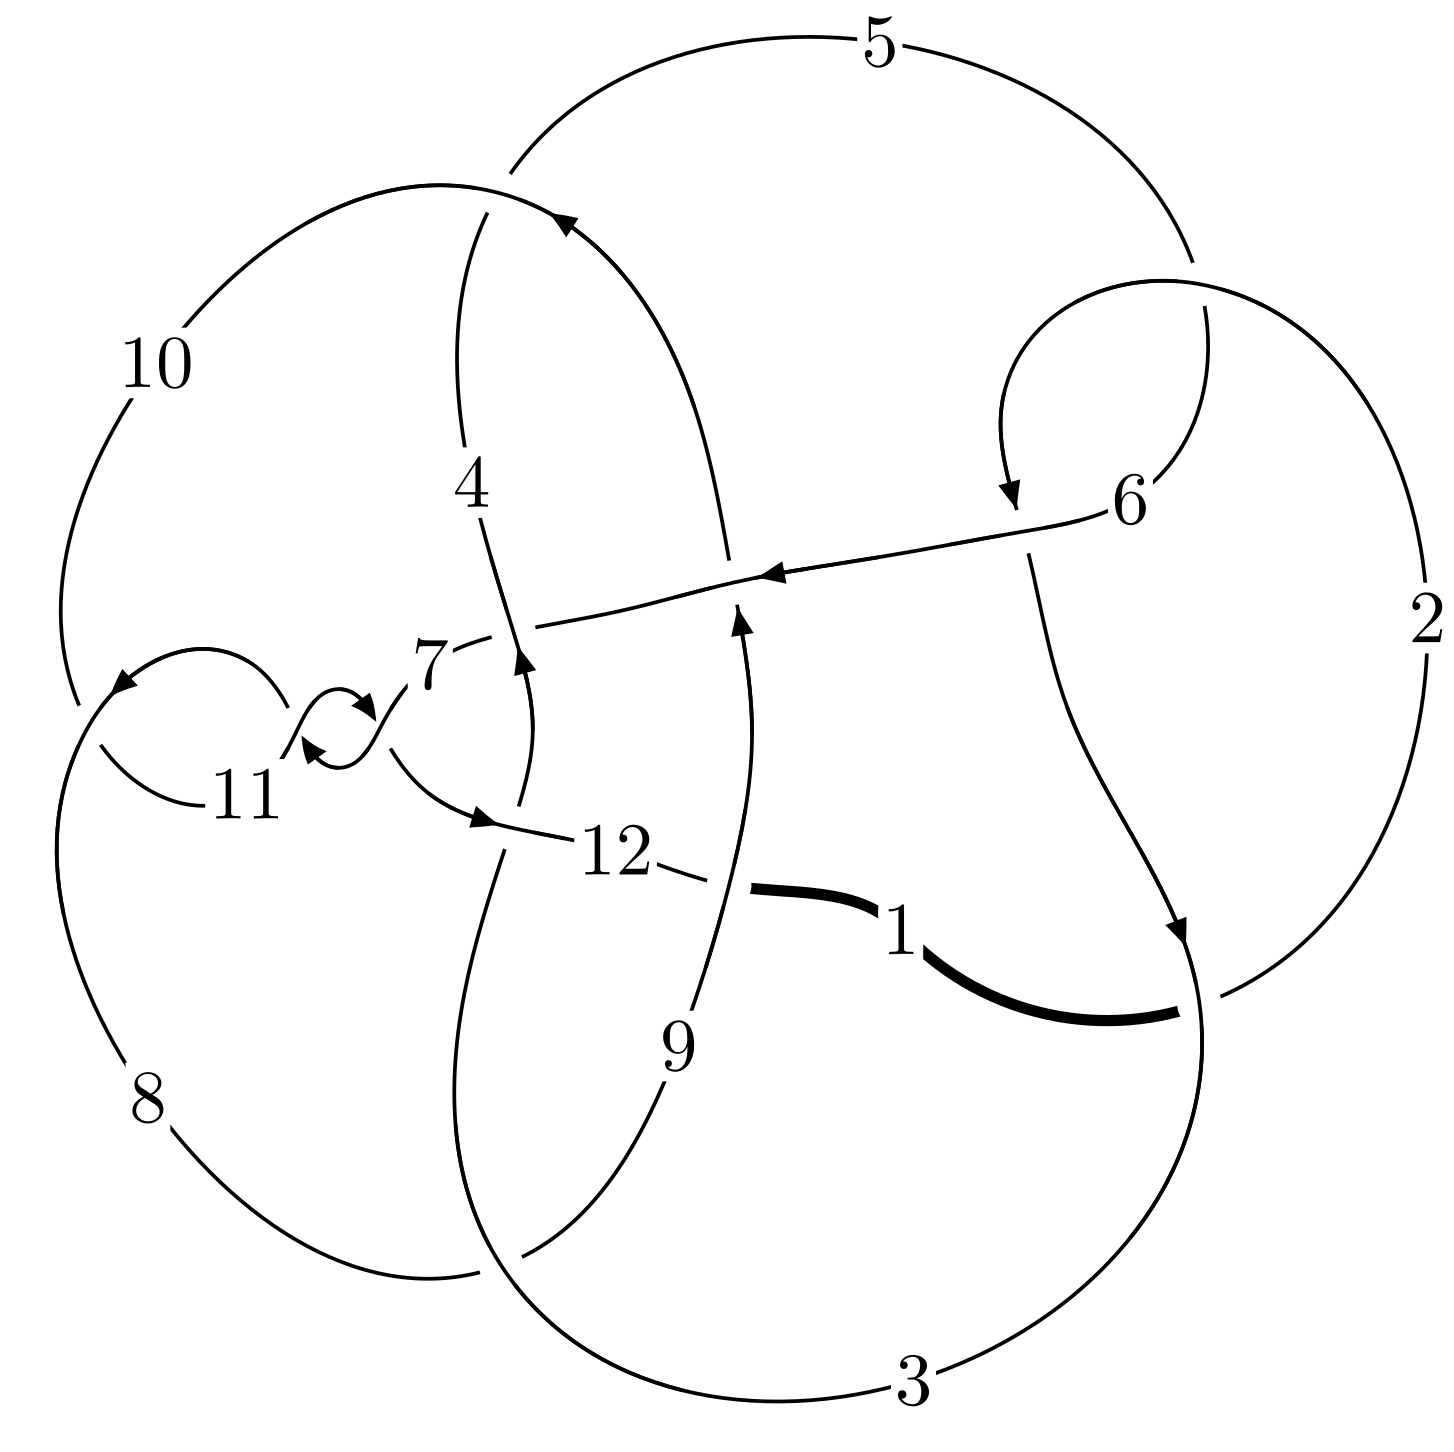
\includegraphics[width=112pt]{../../../GIT/diagram.site/Diagrams/png/2531_12n_0442.png}\\
\ \ \ A knot diagram\footnotemark}&
\allowdisplaybreaks
\textbf{Linearized knot diagam} \\
\cline{2-2}
 &
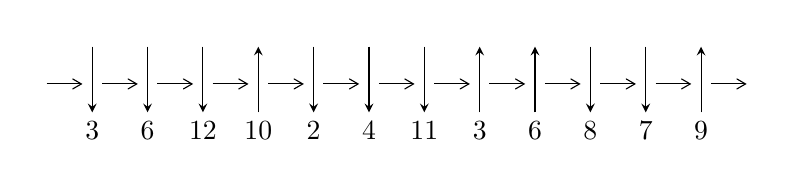
\begin{tikzpicture}[x=20pt, y=17pt]
	% nodes
	\node (C0) at (0, 0) {};
	\node (C1) at (1, 0) {};
	\node (C1U) at (1, +1) {};
	\node (C1D) at (1, -1) {3};

	\node (C2) at (2, 0) {};
	\node (C2U) at (2, +1) {};
	\node (C2D) at (2, -1) {6};

	\node (C3) at (3, 0) {};
	\node (C3U) at (3, +1) {};
	\node (C3D) at (3, -1) {12};

	\node (C4) at (4, 0) {};
	\node (C4U) at (4, +1) {};
	\node (C4D) at (4, -1) {10};

	\node (C5) at (5, 0) {};
	\node (C5U) at (5, +1) {};
	\node (C5D) at (5, -1) {2};

	\node (C6) at (6, 0) {};
	\node (C6U) at (6, +1) {};
	\node (C6D) at (6, -1) {4};

	\node (C7) at (7, 0) {};
	\node (C7U) at (7, +1) {};
	\node (C7D) at (7, -1) {11};

	\node (C8) at (8, 0) {};
	\node (C8U) at (8, +1) {};
	\node (C8D) at (8, -1) {3};

	\node (C9) at (9, 0) {};
	\node (C9U) at (9, +1) {};
	\node (C9D) at (9, -1) {6};

	\node (C10) at (10, 0) {};
	\node (C10U) at (10, +1) {};
	\node (C10D) at (10, -1) {8};

	\node (C11) at (11, 0) {};
	\node (C11U) at (11, +1) {};
	\node (C11D) at (11, -1) {7};

	\node (C12) at (12, 0) {};
	\node (C12U) at (12, +1) {};
	\node (C12D) at (12, -1) {9};
	\node (C13) at (13, 0) {};

	% arrows
	\draw[->,>={angle 60}]
	(C0) edge (C1) (C1) edge (C2) (C2) edge (C3) (C3) edge (C4) (C4) edge (C5) (C5) edge (C6) (C6) edge (C7) (C7) edge (C8) (C8) edge (C9) (C9) edge (C10) (C10) edge (C11) (C11) edge (C12) (C12) edge (C13) ;	\draw[->,>=stealth]
	(C1U) edge (C1D) (C2U) edge (C2D) (C3U) edge (C3D) (C4D) edge (C4U) (C5U) edge (C5D) (C6U) edge (C6D) (C7U) edge (C7D) (C8D) edge (C8U) (C9D) edge (C9U) (C10U) edge (C10D) (C11U) edge (C11D) (C12D) edge (C12U) ;
	\end{tikzpicture} \\
\hhline{~~} \\& 
\textbf{Solving Sequence} \\ \cline{2-2} 
 &
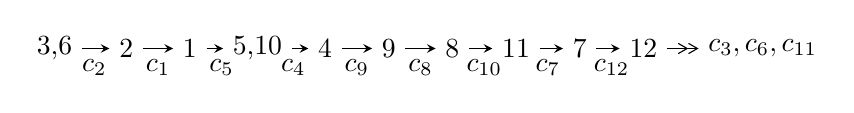
\begin{tikzpicture}[x=23pt, y=7pt]
	% node
	\node (A0) at (-1/8, 0) {3,6};
	\node (A1) at (1, 0) {2};
	\node (A2) at (2, 0) {1};
	\node (A3) at (49/16, 0) {5,10};
	\node (A4) at (33/8, 0) {4};
	\node (A5) at (41/8, 0) {9};
	\node (A6) at (49/8, 0) {8};
	\node (A7) at (57/8, 0) {11};
	\node (A8) at (65/8, 0) {7};
	\node (A9) at (73/8, 0) {12};
	\node (C1) at (1/2, -1) {$c_{2}$};
	\node (C2) at (3/2, -1) {$c_{1}$};
	\node (C3) at (5/2, -1) {$c_{5}$};
	\node (C4) at (29/8, -1) {$c_{4}$};
	\node (C5) at (37/8, -1) {$c_{9}$};
	\node (C6) at (45/8, -1) {$c_{8}$};
	\node (C7) at (53/8, -1) {$c_{10}$};
	\node (C8) at (61/8, -1) {$c_{7}$};
	\node (C9) at (69/8, -1) {$c_{12}$};
	\node (A10) at (11, 0) {$c_{3},c_{6},c_{11}$};

	% edge
	\draw[->,>=stealth]	
	(A0) edge (A1) (A1) edge (A2) (A2) edge (A3) (A3) edge (A4) (A4) edge (A5) (A5) edge (A6) (A6) edge (A7) (A7) edge (A8) (A8) edge (A9) ;
	\draw[->>,>={angle 60}]	
	(A9) edge (A10);
\end{tikzpicture} \\ 

\end{tabular} \\

\footnotetext{
The image of knot diagram is generated by the software ``\textbf{Draw programme}" developed by Andrew Bartholomew(\url{http://www.layer8.co.uk/maths/draw/index.htm\#Running-draw}), where we modified some parts for our purpose(\url{https://github.com/CATsTAILs/LinksPainter}).
}\phantom \\ \newline 
\centering \textbf{Ideals for irreducible components\footnotemark of $X_{\text{par}}$} 
 
\begin{align*}
I^u_{1}&=\langle 
191026393 u^{16}-1652039068 u^{15}+\cdots+64719689 b+1958494945,\\
\phantom{I^u_{1}}&\phantom{= \langle  }-1223765713 u^{16}+10597268099 u^{15}+\cdots+1553272536 a-9878621497,\\
\phantom{I^u_{1}}&\phantom{= \langle  }u^{17}-11 u^{16}+\cdots+25 u-24\rangle \\
I^u_{2}&=\langle 
- u^9-5 u^8-6 u^7+8 u^6+25 u^5+16 u^4-11 u^3-14 u^2+b+u+7,\\
\phantom{I^u_{2}}&\phantom{= \langle  }-7 u^9-51 u^8-149 u^7-213 u^6-119 u^5+61 u^4+107 u^3+8 u^2+5 a-56 u-27,\\
\phantom{I^u_{2}}&\phantom{= \langle  }u^{10}+8 u^9+27 u^8+49 u^7+47 u^6+12 u^5-21 u^4-19 u^3+3 u^2+11 u+5\rangle \\
I^u_{3}&=\langle 
- u^8 a+2 u^8+\cdots- a-4,\;- u^8 a- u^8+\cdots+a^2+4,\;u^9+4 u^8+u^7-9 u^6+12 u^4+2 u^3+4 u^2+1\rangle \\
I^u_{4}&=\langle 
b^4-2 b^3+3 b^2-2 b+3,\;a+1,\;u-1\rangle \\
I^u_{5}&=\langle 
b^2+b+1,\;a-1,\;u-1\rangle \\
\\
\end{align*}
\raggedright * 5 irreducible components of $\dim_{\mathbb{C}}=0$, with total 51 representations.\\
\footnotetext{All coefficients of polynomials are rational numbers. But the coefficients are sometimes approximated in decimal forms when there is not enough margin.}
\newpage
\renewcommand{\arraystretch}{1}
\centering \section*{I. $I^u_{1}= \langle 1.91\times10^{8} u^{16}-1.65\times10^{9} u^{15}+\cdots+6.47\times10^{7} b+1.96\times10^{9},\;-1.22\times10^{9} u^{16}+1.06\times10^{10} u^{15}+\cdots+1.55\times10^{9} a-9.88\times10^{9},\;u^{17}-11 u^{16}+\cdots+25 u-24 \rangle$}
\flushleft \textbf{(i) Arc colorings}\\
\begin{tabular}{m{7pt} m{180pt} m{7pt} m{180pt} }
\flushright $a_{3}=$&$\begin{pmatrix}1\\0\end{pmatrix}$ \\
\flushright $a_{6}=$&$\begin{pmatrix}0\\u\end{pmatrix}$ \\
\flushright $a_{2}=$&$\begin{pmatrix}1\\- u^2\end{pmatrix}$ \\
\flushright $a_{1}=$&$\begin{pmatrix}- u^2+1\\- u^2\end{pmatrix}$ \\
\flushright $a_{5}=$&$\begin{pmatrix}u\\- u^3+u\end{pmatrix}$ \\
\flushright $a_{10}=$&$\begin{pmatrix}0.787863 u^{16}-6.82254 u^{15}+\cdots-4.19484 u+6.35988\\-2.95160 u^{16}+25.5261 u^{15}+\cdots+20.2471 u-30.2612\end{pmatrix}$ \\
\flushright $a_{4}=$&$\begin{pmatrix}-0.502780 u^{16}+4.36822 u^{15}+\cdots+2.45724 u-4.87506\\1.68304 u^{16}-14.9279 u^{15}+\cdots-10.7408 u+18.8611\end{pmatrix}$ \\
\flushright $a_{9}=$&$\begin{pmatrix}0.787863 u^{16}-6.82254 u^{15}+\cdots-4.19484 u+6.35988\\1.37093 u^{16}-11.8653 u^{15}+\cdots-6.94294 u+13.9936\end{pmatrix}$ \\
\flushright $a_{8}=$&$\begin{pmatrix}-0.583066 u^{16}+5.04279 u^{15}+\cdots+2.74810 u-7.63370\\1.37093 u^{16}-11.8653 u^{15}+\cdots-6.94294 u+13.9936\end{pmatrix}$ \\
\flushright $a_{11}=$&$\begin{pmatrix}-0.149136 u^{16}+1.25050 u^{15}+\cdots+3.19107 u-2.49878\\-0.717661 u^{16}+6.21375 u^{15}+\cdots+5.68076 u-7.77323\end{pmatrix}$ \\
\flushright $a_{7}=$&$\begin{pmatrix}-0.785878 u^{16}+6.96162 u^{15}+\cdots+3.90013 u-8.90611\\-0.0529908 u^{16}+0.408128 u^{15}+\cdots+0.448137 u-0.173332\end{pmatrix}$ \\
\flushright $a_{12}=$&$\begin{pmatrix}0.659584 u^{16}-5.85549 u^{15}+\cdots-6.23720 u+8.19166\\1.16236 u^{16}-10.2237 u^{15}+\cdots-7.69444 u+12.0667\end{pmatrix}$\\&\end{tabular}
\flushleft \textbf{(ii) Obstruction class $= -1$}\\~\\
\flushleft \textbf{(iii) Cusp Shapes $= \frac{258679440}{64719689} u^{16}-\frac{2255352174}{64719689} u^{15}+\cdots-\frac{1298645313}{64719689} u+\frac{2660816310}{64719689}$}\\~\\
\newpage\renewcommand{\arraystretch}{1}
\flushleft \textbf{(iv) u-Polynomials at the component}\newline \\
\begin{tabular}{m{50pt}|m{274pt}}
Crossings & \hspace{64pt}u-Polynomials at each crossing \\
\hline $$\begin{aligned}c_{1}\end{aligned}$$&$\begin{aligned}
&u^{17}+33 u^{16}+\cdots-5039 u+576
\end{aligned}$\\
\hline $$\begin{aligned}c_{2},c_{5}\end{aligned}$$&$\begin{aligned}
&u^{17}+11 u^{16}+\cdots+25 u+24
\end{aligned}$\\
\hline $$\begin{aligned}c_{3},c_{6}\end{aligned}$$&$\begin{aligned}
&u^{17}- u^{16}+\cdots+4 u+1
\end{aligned}$\\
\hline $$\begin{aligned}c_{4},c_{8}\end{aligned}$$&$\begin{aligned}
&u^{17}+14 u^{15}+\cdots-6 u^2+1
\end{aligned}$\\
\hline $$\begin{aligned}c_{7},c_{10},c_{11}\end{aligned}$$&$\begin{aligned}
&u^{17}-6 u^{16}+\cdots+19 u-2
\end{aligned}$\\
\hline $$\begin{aligned}c_{9},c_{12}\end{aligned}$$&$\begin{aligned}
&u^{17}+u^{16}+\cdots+33 u+3
\end{aligned}$\\
\hline
\end{tabular}\\~\\
\newpage\renewcommand{\arraystretch}{1}
\flushleft \textbf{(v) Riley Polynomials at the component}\newline \\
\begin{tabular}{m{50pt}|m{274pt}}
Crossings & \hspace{64pt}Riley Polynomials at each crossing \\
\hline $$\begin{aligned}c_{1}\end{aligned}$$&$\begin{aligned}
&y^{17}-117 y^{16}+\cdots+20649889 y-331776
\end{aligned}$\\
\hline $$\begin{aligned}c_{2},c_{5}\end{aligned}$$&$\begin{aligned}
&y^{17}-33 y^{16}+\cdots-5039 y-576
\end{aligned}$\\
\hline $$\begin{aligned}c_{3},c_{6}\end{aligned}$$&$\begin{aligned}
&y^{17}+13 y^{16}+\cdots-22 y-1
\end{aligned}$\\
\hline $$\begin{aligned}c_{4},c_{8}\end{aligned}$$&$\begin{aligned}
&y^{17}+28 y^{16}+\cdots+12 y-1
\end{aligned}$\\
\hline $$\begin{aligned}c_{7},c_{10},c_{11}\end{aligned}$$&$\begin{aligned}
&y^{17}+14 y^{16}+\cdots+93 y-4
\end{aligned}$\\
\hline $$\begin{aligned}c_{9},c_{12}\end{aligned}$$&$\begin{aligned}
&y^{17}+35 y^{16}+\cdots+1875 y-9
\end{aligned}$\\
\hline
\end{tabular}\\~\\
\newpage\flushleft \textbf{(vi) Complex Volumes and Cusp Shapes}
$$\begin{array}{c|c|c}  
\text{Solutions to }I^u_{1}& \I (\text{vol} + \sqrt{-1}CS) & \text{Cusp shape}\\
 \hline 
\begin{aligned}
u &= -0.942057 + 0.494267 I \\
a &= -0.753350 - 0.421156 I \\
b &= \phantom{-}0.435867 - 0.555452 I\end{aligned}
 & \phantom{-}1.96186 + 2.24541 I & \phantom{-}1.44074 - 2.23530 I \\ \hline\begin{aligned}
u &= -0.942057 - 0.494267 I \\
a &= -0.753350 + 0.421156 I \\
b &= \phantom{-}0.435867 + 0.555452 I\end{aligned}
 & \phantom{-}1.96186 - 2.24541 I & \phantom{-}1.44074 + 2.23530 I \\ \hline\begin{aligned}
u &= \phantom{-}1.095620 + 0.300147 I \\
a &= \phantom{-}0.131673 - 0.311290 I \\
b &= -1.033950 - 0.750497 I\end{aligned}
 & \phantom{-}2.79366 + 0.08444 I & -4.63288 + 0.68709 I \\ \hline\begin{aligned}
u &= \phantom{-}1.095620 - 0.300147 I \\
a &= \phantom{-}0.131673 + 0.311290 I \\
b &= -1.033950 + 0.750497 I\end{aligned}
 & \phantom{-}2.79366 - 0.08444 I & -4.63288 - 0.68709 I \\ \hline\begin{aligned}
u &= \phantom{-}0.836685\phantom{ +0.000000I} \\
a &= -0.0818231\phantom{ +0.000000I} \\
b &= \phantom{-}0.476471\phantom{ +0.000000I}\end{aligned}
 & -1.37068\phantom{ +0.000000I} & -8.35980\phantom{ +0.000000I} \\ \hline\begin{aligned}
u &= -0.320479 + 0.572318 I \\
a &= \phantom{-}0.08297 + 1.68332 I \\
b &= -0.103629 + 0.996127 I\end{aligned}
 & \phantom{-}7.44498 + 0.11919 I & \phantom{-}3.63980 - 1.93920 I \\ \hline\begin{aligned}
u &= -0.320479 - 0.572318 I \\
a &= \phantom{-}0.08297 - 1.68332 I \\
b &= -0.103629 - 0.996127 I\end{aligned}
 & \phantom{-}7.44498 - 0.11919 I & \phantom{-}3.63980 + 1.93920 I \\ \hline\begin{aligned}
u &= -1.25347 + 0.91415 I \\
a &= \phantom{-}0.916560 - 0.265291 I \\
b &= \phantom{-}0.46012 + 1.98973 I\end{aligned}
 & \phantom{-}5.01538 + 5.62718 I & -1.75252 - 3.01899 I \\ \hline\begin{aligned}
u &= -1.25347 - 0.91415 I \\
a &= \phantom{-}0.916560 + 0.265291 I \\
b &= \phantom{-}0.46012 - 1.98973 I\end{aligned}
 & \phantom{-}5.01538 - 5.62718 I & -1.75252 + 3.01899 I \\ \hline\begin{aligned}
u &= -0.032060 + 0.412278 I \\
a &= -1.57998 - 0.21566 I \\
b &= -0.592975 + 0.413733 I\end{aligned}
 & \phantom{-}0.026615 - 1.286250 I & \phantom{-}0.68462 + 4.17584 I\\
 \hline 
 \end{array}$$\newpage$$\begin{array}{c|c|c}  
\text{Solutions to }I^u_{1}& \I (\text{vol} + \sqrt{-1}CS) & \text{Cusp shape}\\
 \hline 
\begin{aligned}
u &= -0.032060 - 0.412278 I \\
a &= -1.57998 + 0.21566 I \\
b &= -0.592975 - 0.413733 I\end{aligned}
 & \phantom{-}0.026615 + 1.286250 I & \phantom{-}0.68462 - 4.17584 I \\ \hline\begin{aligned}
u &= \phantom{-}2.13442 + 0.33433 I \\
a &= -0.041538 + 1.111040 I \\
b &= \phantom{-}1.96060 - 2.85602 I\end{aligned}
 & -10.20570 - 0.23808 I & -2.00230 - 0.80635 I \\ \hline\begin{aligned}
u &= \phantom{-}2.13442 - 0.33433 I \\
a &= -0.041538 - 1.111040 I \\
b &= \phantom{-}1.96060 + 2.85602 I\end{aligned}
 & -10.20570 + 0.23808 I & -2.00230 + 0.80635 I \\ \hline\begin{aligned}
u &= \phantom{-}2.15252 + 0.26857 I \\
a &= \phantom{-}0.260975 - 1.202630 I \\
b &= -2.33574 + 2.94126 I\end{aligned}
 & -7.3294 - 12.2045 I & -2.87951 + 5.29191 I \\ \hline\begin{aligned}
u &= \phantom{-}2.15252 - 0.26857 I \\
a &= \phantom{-}0.260975 + 1.202630 I \\
b &= -2.33574 - 2.94126 I\end{aligned}
 & -7.3294 + 12.2045 I & -2.87951 - 5.29191 I \\ \hline\begin{aligned}
u &= \phantom{-}2.24717 + 0.01207 I \\
a &= -0.122236 + 1.201380 I \\
b &= \phantom{-}0.47148 - 3.89441 I\end{aligned}
 & -13.0039 - 6.5145 I & -5.31806 + 4.17343 I \\ \hline\begin{aligned}
u &= \phantom{-}2.24717 - 0.01207 I \\
a &= -0.122236 - 1.201380 I \\
b &= \phantom{-}0.47148 + 3.89441 I\end{aligned}
 & -13.0039 + 6.5145 I & -5.31806 - 4.17343 I\\
 \hline 
 \end{array}$$\newpage\newpage\renewcommand{\arraystretch}{1}
\centering \section*{II. $I^u_{2}= \langle - u^9-5 u^8+\cdots+b+7,\;-7 u^9-51 u^8+\cdots+5 a-27,\;u^{10}+8 u^9+\cdots+11 u+5 \rangle$}
\flushleft \textbf{(i) Arc colorings}\\
\begin{tabular}{m{7pt} m{180pt} m{7pt} m{180pt} }
\flushright $a_{3}=$&$\begin{pmatrix}1\\0\end{pmatrix}$ \\
\flushright $a_{6}=$&$\begin{pmatrix}0\\u\end{pmatrix}$ \\
\flushright $a_{2}=$&$\begin{pmatrix}1\\- u^2\end{pmatrix}$ \\
\flushright $a_{1}=$&$\begin{pmatrix}- u^2+1\\- u^2\end{pmatrix}$ \\
\flushright $a_{5}=$&$\begin{pmatrix}u\\- u^3+u\end{pmatrix}$ \\
\flushright $a_{10}=$&$\begin{pmatrix}\frac{7}{5} u^9+\frac{51}{5} u^8+\cdots+\frac{56}{5} u+\frac{27}{5}\\u^9+5 u^8+6 u^7-8 u^6-25 u^5-16 u^4+11 u^3+14 u^2- u-7\end{pmatrix}$ \\
\flushright $a_{4}=$&$\begin{pmatrix}\frac{4}{5} u^9+\frac{27}{5} u^8+\cdots+\frac{32}{5} u+\frac{9}{5}\\- u^9-8 u^8-26 u^7-43 u^6-33 u^5+3 u^4+24 u^3+10 u^2-9 u-9\end{pmatrix}$ \\
\flushright $a_{9}=$&$\begin{pmatrix}\frac{7}{5} u^9+\frac{51}{5} u^8+\cdots+\frac{56}{5} u+\frac{27}{5}\\u^9+6 u^8+13 u^7+10 u^6-5 u^5-12 u^4- u^3+7 u^2+3 u-2\end{pmatrix}$ \\
\flushright $a_{8}=$&$\begin{pmatrix}\frac{2}{5} u^9+\frac{21}{5} u^8+\cdots+\frac{41}{5} u+\frac{37}{5}\\u^9+6 u^8+13 u^7+10 u^6-5 u^5-12 u^4- u^3+7 u^2+3 u-2\end{pmatrix}$ \\
\flushright $a_{11}=$&$\begin{pmatrix}\frac{13}{5} u^9+\frac{89}{5} u^8+\cdots+\frac{84}{5} u+\frac{23}{5}\\- u^9-9 u^8-33 u^7-61 u^6-52 u^5+2 u^4+38 u^3+16 u^2-15 u-13\end{pmatrix}$ \\
\flushright $a_{7}=$&$\begin{pmatrix}-\frac{9}{5} u^9-\frac{67}{5} u^8+\cdots-\frac{77}{5} u-\frac{54}{5}\\-2 u^9-13 u^8-33 u^7-39 u^6-12 u^5+21 u^4+18 u^3-4 u^2-11 u-1\end{pmatrix}$ \\
\flushright $a_{12}=$&$\begin{pmatrix}\frac{1}{5} u^9+\frac{8}{5} u^8+\cdots+\frac{8}{5} u+\frac{16}{5}\\u^9+7 u^8+20 u^7+29 u^6+18 u^5-6 u^4-15 u^3-4 u^2+7 u+4\end{pmatrix}$\\&\end{tabular}
\flushleft \textbf{(ii) Obstruction class $= 1$}\\~\\
\flushleft \textbf{(iii) Cusp Shapes $= -8 u^9-57 u^8-163 u^7-230 u^6-130 u^5+61 u^4+115 u^3+15 u^2-61 u-34$}\\~\\
\newpage\renewcommand{\arraystretch}{1}
\flushleft \textbf{(iv) u-Polynomials at the component}\newline \\
\begin{tabular}{m{50pt}|m{274pt}}
Crossings & \hspace{64pt}u-Polynomials at each crossing \\
\hline $$\begin{aligned}c_{1}\end{aligned}$$&$\begin{aligned}
&u^{10}-10 u^9+\cdots-91 u+25
\end{aligned}$\\
\hline $$\begin{aligned}c_{2}\end{aligned}$$&$\begin{aligned}
&u^{10}+8 u^9+\cdots+11 u+5
\end{aligned}$\\
\hline $$\begin{aligned}c_{3},c_{6}\end{aligned}$$&$\begin{aligned}
&u^{10}+u^9+3 u^8+u^6-3 u^5-2 u^4- u^3+2 u+1
\end{aligned}$\\
\hline $$\begin{aligned}c_{4},c_{8}\end{aligned}$$&$\begin{aligned}
&u^{10}+6 u^8+7 u^6-2 u^5+5 u^4+2 u^3+5 u^2+2 u+1
\end{aligned}$\\
\hline $$\begin{aligned}c_{5}\end{aligned}$$&$\begin{aligned}
&u^{10}-8 u^9+\cdots-11 u+5
\end{aligned}$\\
\hline $$\begin{aligned}c_{7}\end{aligned}$$&$\begin{aligned}
&u^{10}-3 u^9+\cdots-10 u+3
\end{aligned}$\\
\hline $$\begin{aligned}c_{9},c_{12}\end{aligned}$$&$\begin{aligned}
&u^{10}- u^9+6 u^8-10 u^7+10 u^6-6 u^5+2 u^4- u^3+2 u^2- u+1
\end{aligned}$\\
\hline $$\begin{aligned}c_{10},c_{11}\end{aligned}$$&$\begin{aligned}
&u^{10}+3 u^9+\cdots+10 u+3
\end{aligned}$\\
\hline
\end{tabular}\\~\\
\newpage\renewcommand{\arraystretch}{1}
\flushleft \textbf{(v) Riley Polynomials at the component}\newline \\
\begin{tabular}{m{50pt}|m{274pt}}
Crossings & \hspace{64pt}Riley Polynomials at each crossing \\
\hline $$\begin{aligned}c_{1}\end{aligned}$$&$\begin{aligned}
&y^{10}-22 y^9+\cdots+2569 y+625
\end{aligned}$\\
\hline $$\begin{aligned}c_{2},c_{5}\end{aligned}$$&$\begin{aligned}
&y^{10}-10 y^9+\cdots-91 y+25
\end{aligned}$\\
\hline $$\begin{aligned}c_{3},c_{6}\end{aligned}$$&$\begin{aligned}
&y^{10}+5 y^9+11 y^8+8 y^7-9 y^6-15 y^5+4 y^4+13 y^3-4 y+1
\end{aligned}$\\
\hline $$\begin{aligned}c_{4},c_{8}\end{aligned}$$&$\begin{aligned}
&y^{10}+12 y^9+\cdots+6 y+1
\end{aligned}$\\
\hline $$\begin{aligned}c_{7},c_{10},c_{11}\end{aligned}$$&$\begin{aligned}
&y^{10}+9 y^9+\cdots+20 y+9
\end{aligned}$\\
\hline $$\begin{aligned}c_{9},c_{12}\end{aligned}$$&$\begin{aligned}
&y^{10}+11 y^9+36 y^8+12 y^7+6 y^6+8 y^5+24 y^4+15 y^3+6 y^2+3 y+1
\end{aligned}$\\
\hline
\end{tabular}\\~\\
\newpage\flushleft \textbf{(vi) Complex Volumes and Cusp Shapes}
$$\begin{array}{c|c|c}  
\text{Solutions to }I^u_{2}& \I (\text{vol} + \sqrt{-1}CS) & \text{Cusp shape}\\
 \hline 
\begin{aligned}
u &= -0.698244 + 0.611679 I \\
a &= -0.594983 + 0.452728 I \\
b &= -1.12357 - 1.18282 I\end{aligned}
 & \phantom{-}6.61177 + 7.24611 I & \phantom{-}1.48024 - 6.55546 I \\ \hline\begin{aligned}
u &= -0.698244 - 0.611679 I \\
a &= -0.594983 - 0.452728 I \\
b &= -1.12357 + 1.18282 I\end{aligned}
 & \phantom{-}6.61177 - 7.24611 I & \phantom{-}1.48024 + 6.55546 I \\ \hline\begin{aligned}
u &= -0.765895 + 0.862612 I \\
a &= \phantom{-}0.577252 + 0.100829 I \\
b &= \phantom{-}0.25692 + 1.47319 I\end{aligned}
 & \phantom{-}1.12408 + 3.31101 I & -1.94210 - 5.90631 I \\ \hline\begin{aligned}
u &= -0.765895 - 0.862612 I \\
a &= \phantom{-}0.577252 - 0.100829 I \\
b &= \phantom{-}0.25692 - 1.47319 I\end{aligned}
 & \phantom{-}1.12408 - 3.31101 I & -1.94210 + 5.90631 I \\ \hline\begin{aligned}
u &= \phantom{-}0.649524 + 0.270637 I \\
a &= \phantom{-}0.986717 + 0.863844 I \\
b &= \phantom{-}0.280240 - 0.198619 I\end{aligned}
 & -0.88058 + 1.43796 I & -7.95798 - 4.23415 I \\ \hline\begin{aligned}
u &= \phantom{-}0.649524 - 0.270637 I \\
a &= \phantom{-}0.986717 - 0.863844 I \\
b &= \phantom{-}0.280240 + 0.198619 I\end{aligned}
 & -0.88058 - 1.43796 I & -7.95798 + 4.23415 I \\ \hline\begin{aligned}
u &= -1.11228 + 0.88745 I \\
a &= -0.346880 - 0.585052 I \\
b &= \phantom{-}1.56427 - 1.47362 I\end{aligned}
 & \phantom{-}5.04002 - 1.56785 I & -0.680979 + 1.239329 I \\ \hline\begin{aligned}
u &= -1.11228 - 0.88745 I \\
a &= -0.346880 + 0.585052 I \\
b &= \phantom{-}1.56427 + 1.47362 I\end{aligned}
 & \phantom{-}5.04002 + 1.56785 I & -0.680979 - 1.239329 I \\ \hline\begin{aligned}
u &= -2.07310 + 0.22780 I \\
a &= \phantom{-}0.077895 + 1.141750 I \\
b &= -1.47786 - 2.59954 I\end{aligned}
 & -11.89530 + 1.62532 I & -4.89918 - 0.65986 I \\ \hline\begin{aligned}
u &= -2.07310 - 0.22780 I \\
a &= \phantom{-}0.077895 - 1.141750 I \\
b &= -1.47786 + 2.59954 I\end{aligned}
 & -11.89530 - 1.62532 I & -4.89918 + 0.65986 I\\
 \hline 
 \end{array}$$\newpage\newpage\renewcommand{\arraystretch}{1}
\centering \section*{III. $I^u_{3}= \langle - u^8 a+2 u^8+\cdots- a-4,\;- u^8 a- u^8+\cdots+a^2+4,\;u^9+4 u^8+u^7-9 u^6+12 u^4+2 u^3+4 u^2+1 \rangle$}
\flushleft \textbf{(i) Arc colorings}\\
\begin{tabular}{m{7pt} m{180pt} m{7pt} m{180pt} }
\flushright $a_{3}=$&$\begin{pmatrix}1\\0\end{pmatrix}$ \\
\flushright $a_{6}=$&$\begin{pmatrix}0\\u\end{pmatrix}$ \\
\flushright $a_{2}=$&$\begin{pmatrix}1\\- u^2\end{pmatrix}$ \\
\flushright $a_{1}=$&$\begin{pmatrix}- u^2+1\\- u^2\end{pmatrix}$ \\
\flushright $a_{5}=$&$\begin{pmatrix}u\\- u^3+u\end{pmatrix}$ \\
\flushright $a_{10}=$&$\begin{pmatrix}a\\\frac{1}{8} u^8 a-\frac{1}{4} u^8+\cdots+\frac{1}{8} a+\frac{1}{2}\end{pmatrix}$ \\
\flushright $a_{4}=$&$\begin{pmatrix}-\frac{1}{4} u^8 a+\frac{7}{8} u^8+\cdots+\frac{1}{2} a+\frac{15}{8}\\\frac{1}{4} u^8 a+\frac{3}{8} u^8+\cdots+\frac{1}{2} a-\frac{5}{8}\end{pmatrix}$ \\
\flushright $a_{9}=$&$\begin{pmatrix}a\\\frac{1}{8} u^8 a-\frac{1}{4} u^8+\cdots+\frac{1}{8} a+\frac{1}{2}\end{pmatrix}$ \\
\flushright $a_{8}=$&$\begin{pmatrix}-\frac{1}{8} u^8 a+\frac{1}{4} u^8+\cdots+\frac{7}{8} a-\frac{1}{2}\\\frac{1}{8} u^8 a-\frac{1}{4} u^8+\cdots+\frac{1}{8} a+\frac{1}{2}\end{pmatrix}$ \\
\flushright $a_{11}=$&$\begin{pmatrix}-\frac{1}{4} u^8 a+\frac{1}{2} u^8+\cdots+\frac{1}{2} a+\frac{5}{4}\\\frac{1}{8} u^8 a-\frac{3}{4} u^8+\cdots+\frac{3}{8} a-\frac{3}{4}\end{pmatrix}$ \\
\flushright $a_{7}=$&$\begin{pmatrix}-\frac{1}{2} u^8 a-\frac{7}{8} u^8+\cdots-\frac{1}{4} a-\frac{7}{8}\\\frac{1}{4} u^8 a+\frac{3}{8} u^8+\cdots+\frac{3}{4} a-\frac{3}{8}\end{pmatrix}$ \\
\flushright $a_{12}=$&$\begin{pmatrix}- u^8-4 u^7- u^6+9 u^5-12 u^3-2 u^2-4 u\\\frac{1}{2} u^8 a+\frac{1}{8} u^8+\cdots+\frac{1}{4} a-\frac{7}{8}\end{pmatrix}$\\&\end{tabular}
\flushleft \textbf{(ii) Obstruction class $= -1$}\\~\\
\flushleft \textbf{(iii) Cusp Shapes $= \frac{5}{4} u^8+\frac{25}{4} u^7+\frac{7}{2} u^6-\frac{63}{4} u^5-\frac{15}{4} u^4+\frac{93}{4} u^3+\frac{7}{4} u^2+\frac{27}{4} u-\frac{13}{4}$}\\~\\
\newpage\renewcommand{\arraystretch}{1}
\flushleft \textbf{(iv) u-Polynomials at the component}\newline \\
\begin{tabular}{m{50pt}|m{274pt}}
Crossings & \hspace{64pt}u-Polynomials at each crossing \\
\hline $$\begin{aligned}c_{1}\end{aligned}$$&$\begin{aligned}
&(u^9+14 u^8+73 u^7+173 u^6+188 u^5+80 u^4-74 u^3+40 u^2-8 u+1)^{2}
\end{aligned}$\\
\hline $$\begin{aligned}c_{2},c_{5}\end{aligned}$$&$\begin{aligned}
&(u^9-4 u^8+u^7+9 u^6-12 u^4+2 u^3-4 u^2-1)^2
\end{aligned}$\\
\hline $$\begin{aligned}c_{3},c_{6}\end{aligned}$$&$\begin{aligned}
&u^{18}-4 u^{17}+\cdots-19 u+7
\end{aligned}$\\
\hline $$\begin{aligned}c_{4},c_{8}\end{aligned}$$&$\begin{aligned}
&u^{18}+17 u^{16}+\cdots-33 u+61
\end{aligned}$\\
\hline $$\begin{aligned}c_{7},c_{10},c_{11}\end{aligned}$$&$\begin{aligned}
&(u^9+u^8+5 u^7+4 u^6+8 u^5+5 u^4+3 u^3-2 u-2)^2
\end{aligned}$\\
\hline $$\begin{aligned}c_{9},c_{12}\end{aligned}$$&$\begin{aligned}
&u^{18}-3 u^{17}+\cdots-38 u+787
\end{aligned}$\\
\hline
\end{tabular}\\~\\
\newpage\renewcommand{\arraystretch}{1}
\flushleft \textbf{(v) Riley Polynomials at the component}\newline \\
\begin{tabular}{m{50pt}|m{274pt}}
Crossings & \hspace{64pt}Riley Polynomials at each crossing \\
\hline $$\begin{aligned}c_{1}\end{aligned}$$&$\begin{aligned}
&(y^9-50 y^8+\cdots-16 y-1)^{2}
\end{aligned}$\\
\hline $$\begin{aligned}c_{2},c_{5}\end{aligned}$$&$\begin{aligned}
&(y^9-14 y^8+73 y^7-173 y^6+188 y^5-80 y^4-74 y^3-40 y^2-8 y-1)^{2}
\end{aligned}$\\
\hline $$\begin{aligned}c_{3},c_{6}\end{aligned}$$&$\begin{aligned}
&y^{18}+2 y^{17}+\cdots+451 y+49
\end{aligned}$\\
\hline $$\begin{aligned}c_{4},c_{8}\end{aligned}$$&$\begin{aligned}
&y^{18}+34 y^{17}+\cdots+4279 y+3721
\end{aligned}$\\
\hline $$\begin{aligned}c_{7},c_{10},c_{11}\end{aligned}$$&$\begin{aligned}
&(y^9+9 y^8+33 y^7+60 y^6+50 y^5+7 y^4-7 y^3+8 y^2+4 y-4)^2
\end{aligned}$\\
\hline $$\begin{aligned}c_{9},c_{12}\end{aligned}$$&$\begin{aligned}
&y^{18}+29 y^{17}+\cdots+1731530 y+619369
\end{aligned}$\\
\hline
\end{tabular}\\~\\
\newpage\flushleft \textbf{(vi) Complex Volumes and Cusp Shapes}
$$\begin{array}{c|c|c}  
\text{Solutions to }I^u_{3}& \I (\text{vol} + \sqrt{-1}CS) & \text{Cusp shape}\\
 \hline 
\begin{aligned}
u &= \phantom{-}1.149930 + 0.591217 I \\
a &= -0.601255 - 0.402054 I \\
b &= -0.395481 + 0.118419 I\end{aligned}
 & \phantom{-}1.86176 + 1.02570 I & -2.63382 - 1.45009 I \\ \hline\begin{aligned}
u &= \phantom{-}1.149930 + 0.591217 I \\
a &= \phantom{-}1.283380 - 0.095795 I \\
b &= -0.77918 - 2.34414 I\end{aligned}
 & \phantom{-}1.86176 + 1.02570 I & -2.63382 - 1.45009 I \\ \hline\begin{aligned}
u &= \phantom{-}1.149930 - 0.591217 I \\
a &= -0.601255 + 0.402054 I \\
b &= -0.395481 - 0.118419 I\end{aligned}
 & \phantom{-}1.86176 - 1.02570 I & -2.63382 + 1.45009 I \\ \hline\begin{aligned}
u &= \phantom{-}1.149930 - 0.591217 I \\
a &= \phantom{-}1.283380 + 0.095795 I \\
b &= -0.77918 + 2.34414 I\end{aligned}
 & \phantom{-}1.86176 - 1.02570 I & -2.63382 + 1.45009 I \\ \hline\begin{aligned}
u &= -0.256958 + 0.481474 I \\
a &= \phantom{-}2.09172 + 0.18082 I \\
b &= -0.347105 + 0.467672 I\end{aligned}
 & \phantom{-}5.86635 - 5.34937 I & -0.84423 + 2.78056 I \\ \hline\begin{aligned}
u &= -0.256958 + 0.481474 I \\
a &= \phantom{-}0.39890 - 2.37095 I \\
b &= \phantom{-}1.48260 - 1.54705 I\end{aligned}
 & \phantom{-}5.86635 - 5.34937 I & -0.84423 + 2.78056 I \\ \hline\begin{aligned}
u &= -0.256958 - 0.481474 I \\
a &= \phantom{-}2.09172 - 0.18082 I \\
b &= -0.347105 - 0.467672 I\end{aligned}
 & \phantom{-}5.86635 + 5.34937 I & -0.84423 - 2.78056 I \\ \hline\begin{aligned}
u &= -0.256958 - 0.481474 I \\
a &= \phantom{-}0.39890 + 2.37095 I \\
b &= \phantom{-}1.48260 + 1.54705 I\end{aligned}
 & \phantom{-}5.86635 + 5.34937 I & -0.84423 - 2.78056 I \\ \hline\begin{aligned}
u &= \phantom{-}0.202323 + 0.429977 I \\
a &= -1.06958 - 1.32915 I \\
b &= -0.028684 + 0.501202 I\end{aligned}
 & -0.08117 - 1.83340 I & -4.79553 + 3.05314 I \\ \hline\begin{aligned}
u &= \phantom{-}0.202323 + 0.429977 I \\
a &= -1.78447 + 1.20971 I \\
b &= -0.54712 + 1.46919 I\end{aligned}
 & -0.08117 - 1.83340 I & -4.79553 + 3.05314 I\\
 \hline 
 \end{array}$$\newpage$$\begin{array}{c|c|c}  
\text{Solutions to }I^u_{3}& \I (\text{vol} + \sqrt{-1}CS) & \text{Cusp shape}\\
 \hline 
\begin{aligned}
u &= \phantom{-}0.202323 - 0.429977 I \\
a &= -1.06958 + 1.32915 I \\
b &= -0.028684 - 0.501202 I\end{aligned}
 & -0.08117 + 1.83340 I & -4.79553 - 3.05314 I \\ \hline\begin{aligned}
u &= \phantom{-}0.202323 - 0.429977 I \\
a &= -1.78447 - 1.20971 I \\
b &= -0.54712 - 1.46919 I\end{aligned}
 & -0.08117 + 1.83340 I & -4.79553 - 3.05314 I \\ \hline\begin{aligned}
u &= -2.04009 + 0.22792 I \\
a &= -0.374086 - 0.921422 I \\
b &= \phantom{-}2.26253 + 1.38756 I\end{aligned}
 & -10.25890 + 3.35426 I & -1.96692 - 2.76177 I \\ \hline\begin{aligned}
u &= -2.04009 + 0.22792 I \\
a &= -0.189467 + 1.360530 I \\
b &= -0.72311 - 3.40708 I\end{aligned}
 & -10.25890 + 3.35426 I & -1.96692 - 2.76177 I \\ \hline\begin{aligned}
u &= -2.04009 - 0.22792 I \\
a &= -0.374086 + 0.921422 I \\
b &= \phantom{-}2.26253 - 1.38756 I\end{aligned}
 & -10.25890 - 3.35426 I & -1.96692 + 2.76177 I \\ \hline\begin{aligned}
u &= -2.04009 - 0.22792 I \\
a &= -0.189467 - 1.360530 I \\
b &= -0.72311 + 3.40708 I\end{aligned}
 & -10.25890 - 3.35426 I & -1.96692 + 2.76177 I \\ \hline\begin{aligned}
u &= -2.11041\phantom{ +0.000000I} \\
a &= \phantom{-}0.244866 + 1.162790 I \\
b &= -0.92445 - 2.96892 I\end{aligned}
 & -14.5153\phantom{ +0.000000I} & -7.51900\phantom{ +0.000000I} \\ \hline\begin{aligned}
u &= -2.11041\phantom{ +0.000000I} \\
a &= \phantom{-}0.244866 - 1.162790 I \\
b &= -0.92445 + 2.96892 I\end{aligned}
 & -14.5153\phantom{ +0.000000I} & -7.51900\phantom{ +0.000000I}\\
 \hline 
 \end{array}$$\newpage\newpage\renewcommand{\arraystretch}{1}
\centering \section*{IV. $I^u_{4}= \langle b^4-2 b^3+3 b^2-2 b+3,\;a+1,\;u-1 \rangle$}
\flushleft \textbf{(i) Arc colorings}\\
\begin{tabular}{m{7pt} m{180pt} m{7pt} m{180pt} }
\flushright $a_{3}=$&$\begin{pmatrix}1\\0\end{pmatrix}$ \\
\flushright $a_{6}=$&$\begin{pmatrix}0\\1\end{pmatrix}$ \\
\flushright $a_{2}=$&$\begin{pmatrix}1\\-1\end{pmatrix}$ \\
\flushright $a_{1}=$&$\begin{pmatrix}0\\-1\end{pmatrix}$ \\
\flushright $a_{5}=$&$\begin{pmatrix}1\\0\end{pmatrix}$ \\
\flushright $a_{10}=$&$\begin{pmatrix}-1\\b\end{pmatrix}$ \\
\flushright $a_{4}=$&$\begin{pmatrix}- b+1\\b^2\end{pmatrix}$ \\
\flushright $a_{9}=$&$\begin{pmatrix}-1\\b-1\end{pmatrix}$ \\
\flushright $a_{8}=$&$\begin{pmatrix}- b\\b-1\end{pmatrix}$ \\
\flushright $a_{11}=$&$\begin{pmatrix}- b^3+b^2- b-1\\b^3-2 b^2+3 b-1\end{pmatrix}$ \\
\flushright $a_{7}=$&$\begin{pmatrix}- b^2+2 b-1\\b^3- b^2+1\end{pmatrix}$ \\
\flushright $a_{12}=$&$\begin{pmatrix}1\\- b\end{pmatrix}$\\&\end{tabular}
\flushleft \textbf{(ii) Obstruction class $= 1$}\\~\\
\flushleft \textbf{(iii) Cusp Shapes $= 0$}\\~\\
\newpage\renewcommand{\arraystretch}{1}
\flushleft \textbf{(iv) u-Polynomials at the component}\newline \\
\begin{tabular}{m{50pt}|m{274pt}}
Crossings & \hspace{64pt}u-Polynomials at each crossing \\
\hline $$\begin{aligned}c_{1},c_{2}\end{aligned}$$&$\begin{aligned}
&(u-1)^4
\end{aligned}$\\
\hline $$\begin{aligned}c_{3},c_{6}\end{aligned}$$&$\begin{aligned}
&u^4+2 u^3+3 u^2+2 u+3
\end{aligned}$\\
\hline $$\begin{aligned}c_{4},c_{8}\end{aligned}$$&$\begin{aligned}
&u^4-2 u^3+3 u^2-2 u+3
\end{aligned}$\\
\hline $$\begin{aligned}c_{5},c_{9},c_{12}\end{aligned}$$&$\begin{aligned}
&(u+1)^4
\end{aligned}$\\
\hline $$\begin{aligned}c_{7},c_{10},c_{11}\end{aligned}$$&$\begin{aligned}
&(u^2+2)^2
\end{aligned}$\\
\hline
\end{tabular}\\~\\
\newpage\renewcommand{\arraystretch}{1}
\flushleft \textbf{(v) Riley Polynomials at the component}\newline \\
\begin{tabular}{m{50pt}|m{274pt}}
Crossings & \hspace{64pt}Riley Polynomials at each crossing \\
\hline $$\begin{aligned}c_{1},c_{2},c_{5}\\c_{9},c_{12}\end{aligned}$$&$\begin{aligned}
&(y-1)^4
\end{aligned}$\\
\hline $$\begin{aligned}c_{3},c_{4},c_{6}\\c_{8}\end{aligned}$$&$\begin{aligned}
&y^4+2 y^3+7 y^2+14 y+9
\end{aligned}$\\
\hline $$\begin{aligned}c_{7},c_{10},c_{11}\end{aligned}$$&$\begin{aligned}
&(y+2)^4
\end{aligned}$\\
\hline
\end{tabular}\\~\\
\newpage\flushleft \textbf{(vi) Complex Volumes and Cusp Shapes}
$$\begin{array}{c|c|c}  
\text{Solutions to }I^u_{4}& \I (\text{vol} + \sqrt{-1}CS) & \text{Cusp shape}\\
 \hline 
\begin{aligned}
u &= \phantom{-}1.00000\phantom{ +0.000000I} \\
a &= -1.00000\phantom{ +0.000000I} \\
b &= -0.152220 + 1.084150 I\end{aligned}
 & \phantom{-}4.93480\phantom{ +0.000000I} & \phantom{-0.000000 } 0 \\ \hline\begin{aligned}
u &= \phantom{-}1.00000\phantom{ +0.000000I} \\
a &= -1.00000\phantom{ +0.000000I} \\
b &= -0.152220 - 1.084150 I\end{aligned}
 & \phantom{-}4.93480\phantom{ +0.000000I} & \phantom{-0.000000 } 0 \\ \hline\begin{aligned}
u &= \phantom{-}1.00000\phantom{ +0.000000I} \\
a &= -1.00000\phantom{ +0.000000I} \\
b &= \phantom{-}1.15222 + 1.08415 I\end{aligned}
 & \phantom{-}4.93480\phantom{ +0.000000I} & \phantom{-0.000000 } 0 \\ \hline\begin{aligned}
u &= \phantom{-}1.00000\phantom{ +0.000000I} \\
a &= -1.00000\phantom{ +0.000000I} \\
b &= \phantom{-}1.15222 - 1.08415 I\end{aligned}
 & \phantom{-}4.93480\phantom{ +0.000000I} & \phantom{-0.000000 } 0\\
 \hline 
 \end{array}$$\newpage\newpage\renewcommand{\arraystretch}{1}
\centering \section*{V. $I^u_{5}= \langle b^2+b+1,\;a-1,\;u-1 \rangle$}
\flushleft \textbf{(i) Arc colorings}\\
\begin{tabular}{m{7pt} m{180pt} m{7pt} m{180pt} }
\flushright $a_{3}=$&$\begin{pmatrix}1\\0\end{pmatrix}$ \\
\flushright $a_{6}=$&$\begin{pmatrix}0\\1\end{pmatrix}$ \\
\flushright $a_{2}=$&$\begin{pmatrix}1\\-1\end{pmatrix}$ \\
\flushright $a_{1}=$&$\begin{pmatrix}0\\-1\end{pmatrix}$ \\
\flushright $a_{5}=$&$\begin{pmatrix}1\\0\end{pmatrix}$ \\
\flushright $a_{10}=$&$\begin{pmatrix}1\\b\end{pmatrix}$ \\
\flushright $a_{4}=$&$\begin{pmatrix}b+1\\- b-1\end{pmatrix}$ \\
\flushright $a_{9}=$&$\begin{pmatrix}1\\b+1\end{pmatrix}$ \\
\flushright $a_{8}=$&$\begin{pmatrix}- b\\b+1\end{pmatrix}$ \\
\flushright $a_{11}=$&$\begin{pmatrix}1\\b\end{pmatrix}$ \\
\flushright $a_{7}=$&$\begin{pmatrix}- b\\b+1\end{pmatrix}$ \\
\flushright $a_{12}=$&$\begin{pmatrix}1\\b\end{pmatrix}$\\&\end{tabular}
\flushleft \textbf{(ii) Obstruction class $= 1$}\\~\\
\flushleft \textbf{(iii) Cusp Shapes $= -6$}\\~\\
\newpage\renewcommand{\arraystretch}{1}
\flushleft \textbf{(iv) u-Polynomials at the component}\newline \\
\begin{tabular}{m{50pt}|m{274pt}}
Crossings & \hspace{64pt}u-Polynomials at each crossing \\
\hline $$\begin{aligned}c_{1},c_{2},c_{9}\\c_{12}\end{aligned}$$&$\begin{aligned}
&(u-1)^2
\end{aligned}$\\
\hline $$\begin{aligned}c_{3},c_{4},c_{6}\\c_{8}\end{aligned}$$&$\begin{aligned}
&u^2+u+1
\end{aligned}$\\
\hline $$\begin{aligned}c_{5}\end{aligned}$$&$\begin{aligned}
&(u+1)^2
\end{aligned}$\\
\hline $$\begin{aligned}c_{7},c_{10},c_{11}\end{aligned}$$&$\begin{aligned}
&u^2
\end{aligned}$\\
\hline
\end{tabular}\\~\\
\newpage\renewcommand{\arraystretch}{1}
\flushleft \textbf{(v) Riley Polynomials at the component}\newline \\
\begin{tabular}{m{50pt}|m{274pt}}
Crossings & \hspace{64pt}Riley Polynomials at each crossing \\
\hline $$\begin{aligned}c_{1},c_{2},c_{5}\\c_{9},c_{12}\end{aligned}$$&$\begin{aligned}
&(y-1)^2
\end{aligned}$\\
\hline $$\begin{aligned}c_{3},c_{4},c_{6}\\c_{8}\end{aligned}$$&$\begin{aligned}
&y^2+y+1
\end{aligned}$\\
\hline $$\begin{aligned}c_{7},c_{10},c_{11}\end{aligned}$$&$\begin{aligned}
&y^2
\end{aligned}$\\
\hline
\end{tabular}\\~\\
\newpage\flushleft \textbf{(vi) Complex Volumes and Cusp Shapes}
$$\begin{array}{c|c|c}  
\text{Solutions to }I^u_{5}& \I (\text{vol} + \sqrt{-1}CS) & \text{Cusp shape}\\
 \hline 
\begin{aligned}
u &= \phantom{-}1.00000\phantom{ +0.000000I} \\
a &= \phantom{-}1.00000\phantom{ +0.000000I} \\
b &= -0.500000 + 0.866025 I\end{aligned}
 & \phantom{-0.000000 } 0 & -6.00000\phantom{ +0.000000I} \\ \hline\begin{aligned}
u &= \phantom{-}1.00000\phantom{ +0.000000I} \\
a &= \phantom{-}1.00000\phantom{ +0.000000I} \\
b &= -0.500000 - 0.866025 I\end{aligned}
 & \phantom{-0.000000 } 0 & -6.00000\phantom{ +0.000000I}\\
 \hline 
 \end{array}$$\newpage
\newpage\renewcommand{\arraystretch}{1}
\centering \section*{ VI. u-Polynomials}
\begin{tabular}{m{50pt}|m{274pt}}
Crossings & \hspace{64pt}u-Polynomials at each crossing \\
\hline $$\begin{aligned}c_{1}\end{aligned}$$&$\begin{aligned}
&(u-1)^6\\
&\cdot(u^9+14 u^8+73 u^7+173 u^6+188 u^5+80 u^4-74 u^3+40 u^2-8 u+1)^{2}\\
&\cdot(u^{10}-10 u^9+\cdots-91 u+25)(u^{17}+33 u^{16}+\cdots-5039 u+576)
\end{aligned}$\\
\hline $$\begin{aligned}c_{2}\end{aligned}$$&$\begin{aligned}
&(u-1)^6(u^9-4 u^8+u^7+9 u^6-12 u^4+2 u^3-4 u^2-1)^2\\
&\cdot(u^{10}+8 u^9+\cdots+11 u+5)(u^{17}+11 u^{16}+\cdots+25 u+24)
\end{aligned}$\\
\hline $$\begin{aligned}c_{3},c_{6}\end{aligned}$$&$\begin{aligned}
&(u^2+u+1)(u^4+2 u^3+3 u^2+2 u+3)\\
&\cdot(u^{10}+u^9+\cdots+2 u+1)(u^{17}- u^{16}+\cdots+4 u+1)\\
&\cdot(u^{18}-4 u^{17}+\cdots-19 u+7)
\end{aligned}$\\
\hline $$\begin{aligned}c_{4},c_{8}\end{aligned}$$&$\begin{aligned}
&(u^2+u+1)(u^4-2 u^3+3 u^2-2 u+3)\\
&\cdot(u^{10}+6 u^8+7 u^6-2 u^5+5 u^4+2 u^3+5 u^2+2 u+1)\\
&\cdot(u^{17}+14 u^{15}+\cdots-6 u^2+1)(u^{18}+17 u^{16}+\cdots-33 u+61)
\end{aligned}$\\
\hline $$\begin{aligned}c_{5}\end{aligned}$$&$\begin{aligned}
&(u+1)^6(u^9-4 u^8+u^7+9 u^6-12 u^4+2 u^3-4 u^2-1)^2\\
&\cdot(u^{10}-8 u^9+\cdots-11 u+5)(u^{17}+11 u^{16}+\cdots+25 u+24)
\end{aligned}$\\
\hline $$\begin{aligned}c_{7}\end{aligned}$$&$\begin{aligned}
&u^2(u^2+2)^2(u^9+u^8+5 u^7+4 u^6+8 u^5+5 u^4+3 u^3-2 u-2)^2\\
&\cdot(u^{10}-3 u^9+\cdots-10 u+3)(u^{17}-6 u^{16}+\cdots+19 u-2)
\end{aligned}$\\
\hline $$\begin{aligned}c_{9},c_{12}\end{aligned}$$&$\begin{aligned}
&(u-1)^2(u+1)^4\\
&\cdot(u^{10}- u^9+6 u^8-10 u^7+10 u^6-6 u^5+2 u^4- u^3+2 u^2- u+1)\\
&\cdot(u^{17}+u^{16}+\cdots+33 u+3)(u^{18}-3 u^{17}+\cdots-38 u+787)
\end{aligned}$\\
\hline $$\begin{aligned}c_{10},c_{11}\end{aligned}$$&$\begin{aligned}
&u^2(u^2+2)^2(u^9+u^8+5 u^7+4 u^6+8 u^5+5 u^4+3 u^3-2 u-2)^2\\
&\cdot(u^{10}+3 u^9+\cdots+10 u+3)(u^{17}-6 u^{16}+\cdots+19 u-2)
\end{aligned}$\\
\hline
\end{tabular}\newpage\renewcommand{\arraystretch}{1}
\centering \section*{ VII. Riley Polynomials}
\begin{tabular}{m{50pt}|m{274pt}}
Crossings & \hspace{64pt}Riley Polynomials at each crossing \\
\hline $$\begin{aligned}c_{1}\end{aligned}$$&$\begin{aligned}
&((y-1)^6)(y^9-50 y^8+\cdots-16 y-1)^{2}\\
&\cdot(y^{10}-22 y^9+\cdots+2569 y+625)\\
&\cdot(y^{17}-117 y^{16}+\cdots+20649889 y-331776)
\end{aligned}$\\
\hline $$\begin{aligned}c_{2},c_{5}\end{aligned}$$&$\begin{aligned}
&(y-1)^6\\
&\cdot(y^9-14 y^8+73 y^7-173 y^6+188 y^5-80 y^4-74 y^3-40 y^2-8 y-1)^{2}\\
&\cdot(y^{10}-10 y^9+\cdots-91 y+25)(y^{17}-33 y^{16}+\cdots-5039 y-576)
\end{aligned}$\\
\hline $$\begin{aligned}c_{3},c_{6}\end{aligned}$$&$\begin{aligned}
&(y^2+y+1)(y^4+2 y^3+7 y^2+14 y+9)\\
&\cdot(y^{10}+5 y^9+11 y^8+8 y^7-9 y^6-15 y^5+4 y^4+13 y^3-4 y+1)\\
&\cdot(y^{17}+13 y^{16}+\cdots-22 y-1)(y^{18}+2 y^{17}+\cdots+451 y+49)
\end{aligned}$\\
\hline $$\begin{aligned}c_{4},c_{8}\end{aligned}$$&$\begin{aligned}
&(y^2+y+1)(y^4+2 y^3+\cdots+14 y+9)(y^{10}+12 y^9+\cdots+6 y+1)\\
&\cdot(y^{17}+28 y^{16}+\cdots+12 y-1)(y^{18}+34 y^{17}+\cdots+4279 y+3721)
\end{aligned}$\\
\hline $$\begin{aligned}c_{7},c_{10},c_{11}\end{aligned}$$&$\begin{aligned}
&y^2(y+2)^4\\
&\cdot(y^9+9 y^8+33 y^7+60 y^6+50 y^5+7 y^4-7 y^3+8 y^2+4 y-4)^2\\
&\cdot(y^{10}+9 y^9+\cdots+20 y+9)(y^{17}+14 y^{16}+\cdots+93 y-4)
\end{aligned}$\\
\hline $$\begin{aligned}c_{9},c_{12}\end{aligned}$$&$\begin{aligned}
&(y-1)^6\\
&\cdot(y^{10}+11 y^9+36 y^8+12 y^7+6 y^6+8 y^5+24 y^4+15 y^3+6 y^2+3 y+1)\\
&\cdot(y^{17}+35 y^{16}+\cdots+1875 y-9)\\
&\cdot(y^{18}+29 y^{17}+\cdots+1731530 y+619369)
\end{aligned}$\\
\hline
\end{tabular}
\vskip 2pc
\end{document}